\documentclass[aps,prl,twocolumn,superscriptaddress,amsmath,amssymb,10pt]{revtex4-2}
\usepackage{graphicx,bm,amsthm}
\newtheorem{theorem}{Theorem}
\newtheorem{corollary}{Corollary}
\newcommand{\E}{\mathbb{E}}
\newcommand{\Tb}{\overline{T}}
\newcommand{\N}{\mathcal{N}}
\newcommand{\tr}{\operatorname{tr}}

\begin{document}
\title{Scrambled states lose distinguishability exactly at the hashing bound}

\author{Xi Zhao}\noaffiliation
\date{\today}

\begin{abstract}
Two independent random (scrambled) $n$-qubit states that pass through local Pauli noise remain perfectly distinguishable at weak noise and become indistinguishable at strong noise. We prove a two-sided information-spectrum bound: their average trace distance equals, up to corrections $2^{-a}$ and $2^{-a/2}$ with $a\ge0$ arbitrary, the probability that the error string has surprisal $-\log_2 p(P)$ below $n\mp a$. The bound holds for arbitrary, possibly correlated, Pauli noise and needs only state 2-designs. For independent noise, distinguishability therefore undergoes a single sharp transition at the hashing point $H(\bm p)=1$, where the coherent information vanishes. The transition window has width $n^{-1/2}$ and a universal error-function profile. For every noise above threshold, the decay is exponential, so the previously conjectured intermediate regime of algebraic decay does not exist. We derive the decay exponent variationally. It shows a second, freezing-type nonanalyticity, analogous to Derrida's random-energy model, at which the collision-entropy bound first becomes tight.
\end{abstract}
\maketitle

\emph{Introduction.}---Scrambling dynamics spread local information over all degrees of freedom. This makes information robust in some senses and fragile in others. A black hole returns information quickly once it is scrambled~\cite{HaydenPreskill}. Random circuits convert local noise into global white noise~\cite{Dalzell}. Under unital noise, noisy Haar states cannot be told apart from the maximally mixed state by observers without quantum memory~\cite{Bansal}. A basic question underlies all of these statements. Take two scrambled states $\psi_1,\psi_2$ and expose every qubit to noise. How well can an observer with full quantum power still distinguish them? The answer is the Helstrom success probability, set by the trace distance
\begin{equation}
\Tb=\E_{\psi_1,\psi_2}\tfrac12\big\|\N(\psi_1)-\N(\psi_2)\big\|_1 .
\label{eq:T}
\end{equation}
Liu \emph{et al.} recently attacked this question with decoupling techniques~\cite{Liu2026}. For local noise they found a ``resilient'' phase with $\Tb\to1$ below a conditional-entropy threshold and a ``collapsed'' phase with $\Tb\to0$ exponentially above a collision-entropy threshold. For single-qubit depolarizing noise these thresholds are $r\approx0.252$ and $r\approx0.423$. In the interval between them their bounds do not match: the upper bound decays only as $O(n^{-1/2})$, and the structure of this intermediate phase was left as an open problem~\cite{Liu2026}. Spectral studies of Haar-random codes locate a coding transition at the same hashing point, but in terms of entropy densities~\cite{Sommers}.

Here we resolve the problem with an elementary, nonasymptotic two-sided bound, Theorem~1. It identifies $\Tb$ with an information-spectrum quantity, in the spirit of the Verd\'u--Han formula~\cite{VerduHan,HayashiNagaoka}. Three consequences follow for independent noise. (i) There is a single sharp transition, located exactly at the hashing point, where the coherent information $1-H(\bm p)$ of the Pauli channel vanishes~\cite{BDSW,Devetak}. (ii) Near the transition there is universal finite-size scaling with an error-function profile. (iii) Above threshold the decay is exponential, with an exponent bounded by a variational formula. This formula is tight to leading order near threshold and, numerically, everywhere. It also predicts a second, freezing transition, at which the collision-entropy description of Ref.~\cite{Liu2026} first becomes exact.

\emph{Setup.}---Let $d=2^n$ and let $\N(\rho)=\sum_P p(P)\,P\rho P$ be an arbitrary Pauli channel. Here $P$ runs over $n$-qubit Pauli strings and $p$ is any probability distribution, so correlated noise is allowed. We define the surprisal of an error, $s(P)=-\log_2 p(P)$, and regard it as a random variable with $P\sim p$. The states $\psi_{1,2}$ are drawn independently from a state 2-design, for instance Haar-random states or random stabilizer states~\cite{Webb,Zhu}. The averaging in Eq.~\eqref{eq:T} is over this ensemble.

\begin{theorem}
For every Pauli channel and every $a\ge 0$,
\begin{equation}
\Pr[s<n-a]-2^{-a}\;\le\;\Tb\;\le\;\Pr[s<n+a]+\tfrac{1}{\sqrt2}\,2^{-a/2}.
\label{eq:thm}
\end{equation}
More generally, for any set $\mathcal G$ of Pauli strings and any partition of the strings into sets $\{\mathcal C_j\}$,
\begin{equation}
p(\mathcal G)-\frac{|\mathcal G|}{d}\le\Tb\le\sum_j\min\Big\{p(\mathcal C_j),\Big[\frac d2\sum_{P\in\mathcal C_j}p(P)^2\Big]^{1/2}\Big\}.
\label{eq:thm2}
\end{equation}
\end{theorem}

\begin{proof}
\emph{Lower bound.} Fix $\psi_1$ and let $\Pi$ be the projector onto $\mathrm{span}\{P|\psi_1\rangle:P\in\mathcal G\}$, so $\tr\Pi\le|\mathcal G|$. The Helstrom bound gives $\tfrac12\|\N(\psi_1)-\N(\psi_2)\|_1\ge\tr\Pi\,\N(\psi_1)-\tr\Pi\,\N(\psi_2)$. The first term is at least $\sum_{P\in\mathcal G}p(P)=p(\mathcal G)$. Since $\psi_2$ is independent of $\Pi$, averaging the second term over $\psi_2$ uses only the first moment, $\E\,\psi_2=I/d$. This gives $\sum_Q p(Q)\tr(Q\Pi Q)/d=\tr\Pi/d\le|\mathcal G|/d$. To obtain Eq.~\eqref{eq:thm}, choose $\mathcal G=\{s<n-a\}$. Every string in this set has $p(P)>2^{a-n}$, so $|\mathcal G|<2^{n-a}$.

\emph{Upper bound.} Write $\Delta=\psi_1-\psi_2$ and $\N=\sum_j\N_j$, where $\N_j$ keeps only the strings in $\mathcal C_j$. By the triangle inequality, $\tfrac12\|\N(\Delta)\|_1\le\sum_j\tfrac12\|\N_j(\Delta)\|_1$. Each term admits two estimates. First, $\tfrac12\|\N_j(\Delta)\|_1\le p(\mathcal C_j)$, because $\|\Delta\|_1\le2$. Second, by Cauchy--Schwarz and Jensen, $\E\tfrac12\|\N_j(\Delta)\|_1\le\tfrac12[d\,\E\tr\N_j(\Delta)^2]^{1/2}$. The 2-design property gives $\E|\langle\psi|R|\psi\rangle|^2=1/(d+1)$ for every Pauli $R\neq I$. With this one finds
\begin{equation}
\E\tr\N_j(\Delta)^2=\frac{2d}{d+1}\sum_{P\in\mathcal C_j}p(P)^2-\frac{2\,p(\mathcal C_j)^2}{d(d+1)}\le 2\!\sum_{P\in\mathcal C_j}\!p(P)^2 ,
\end{equation}
which proves Eq.~\eqref{eq:thm2}. For Eq.~\eqref{eq:thm}, take two classes, $\{s<n+a\}$ and its complement $\mathcal C$. On $\mathcal C$, $p(P)\le 2^{-n-a}$, so $\sum_{\mathcal C}p^2\le2^{-n-a}$.
\end{proof}

The theorem has a transparent meaning. A $d$-dimensional Hilbert space has room for at most $d$ nearly orthogonal images $P|\psi\rangle$. If the error that occurred is among the $\sim\!2^{n}$ most likely ones ($s<n$), it can be identified and the two scrambled states stay distinguishable. If instead the error belongs to the exponentially large tail of unlikely errors ($s>n$), their images overlap and the distinguishing signal averages out, as in a quantum central-limit theorem. Product states behave very differently. For $|0^n\rangle$ versus the maximally mixed state, the trace distance is $0.44$ already at $r=0.6$, $n=8$, while for Haar states it is $0.10$. The fragility is therefore a property of scrambling, not of the noise strength alone. Note also that the lower bound needs only $\psi_2$ to be a 1-design (with $\psi_1$ arbitrary), and the upper bound needs both states to be 2-designs. All statements below therefore apply verbatim to random stabilizer states.

\emph{Sharp transition at the hashing point.}---Consider independent and identically distributed (i.i.d.) noise, $p=\bm p^{\otimes n}$, with single-qubit distribution $\bm p=(p_0,p_x,p_y,p_z)$, Shannon entropy $H(\bm p)$ (base 2), and variance $\sigma^2(\bm p)$ of $-\log_2 p_i$. Then $s$ is a sum of $n$ i.i.d.\ variables with mean $nH(\bm p)$. We choose $a=n^{1/4}$ in Eq.~\eqref{eq:thm} and apply the Berry--Esseen theorem; with $a=\epsilon n$ we apply Cram\'er's theorem instead. This gives:

\begin{corollary}
If $H(\bm p)<1$, then $\Tb\ge 1-e^{-\Omega(n)}$. If $H(\bm p)>1$, then $\Tb\le e^{-\Omega(n)}$. Along any sequence with $x=\sqrt n\,[1-H(\bm p)]/\sigma(\bm p)$ fixed,
\begin{equation}
\lim_{n\to\infty}\Tb=\Phi(x)=\tfrac12\big[1+\mathrm{erf}(x/\sqrt2)\big].
\label{eq:scaling}
\end{equation}
In particular, $\Tb\to\tfrac12$ exactly at $H(\bm p)=1$.
\end{corollary}

The threshold $H(\bm p)=1$ is precisely the zero of the hashing rate $1-H(\bm p)$, the coherent information of the Pauli channel with maximally mixed input~\cite{BDSW,Devetak}. A pair of scrambled states thus behaves like a logical qubit of a random code~\cite{Liu2026}. It survives exactly when random coding transmits quantum information. For depolarizing noise $\N_r(\rho)=(1-r)\rho+r\,I/2$ (Pauli error probability $q=3r/4$), the threshold is $q_c=0.18929$, i.e., $r_c=0.25239$. This coincides with the resilient-phase boundary of Ref.~\cite{Liu2026}. However, the region $0.252<r<0.423$ is not a separate phase: $\Tb$ decays exponentially there. Figure~\ref{fig:1} illustrates the crossing of all curves at $r_c$ and the collapse onto Eq.~\eqref{eq:scaling}.

\begin{figure}[t]
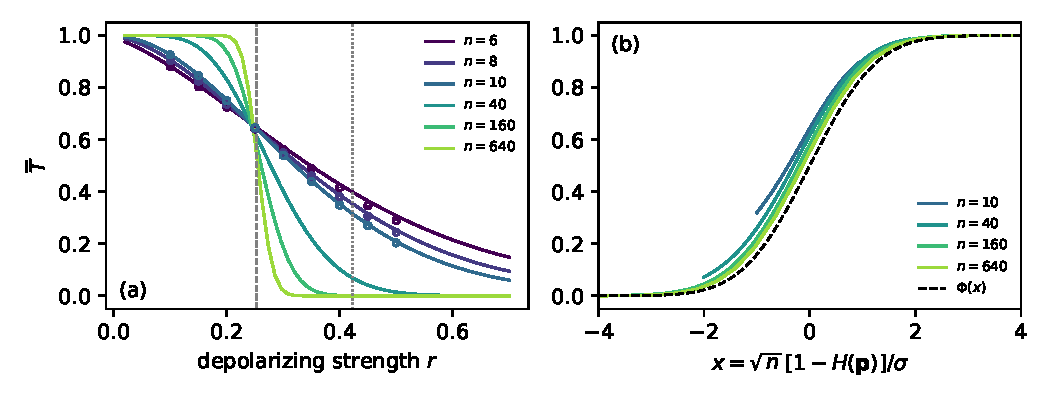
\includegraphics[width=\columnwidth]{fig1.pdf}
\caption{(a) Average trace distance between two Haar states after local depolarizing noise. Symbols: exact density-matrix simulations for $n=6,8$ (40 pairs) and $n=10$ (12 pairs); error bars are standard errors and are mostly smaller than the symbols. Lines: deterministic equivalent, Eq.~\eqref{eq:DE}, for $n=6$--$640$. The dashed line marks the hashing point $r_c=0.252$. The dotted line marks the collision-entropy threshold $r=0.423$ of Ref.~\cite{Liu2026}, which plays no special role. (b) The same data plotted against $x=\sqrt n\,[1-H]/\sigma$ approach the universal profile $\Phi(x)$ (dashed), with corrections $O(\log n/\sqrt n)$.}
\label{fig:1}
\end{figure}

\emph{Decay exponent and freezing.}---Group the Pauli strings into type classes $\mathcal C_t$ according to their empirical distribution $t$ over $\{0,x,y,z\}$. A class has $|\mathcal C_t|\doteq2^{nH(t)}$ elements and total weight $p(\mathcal C_t)\le2^{-nD(t\|\bm p)}$, where $D$ is the relative entropy. All strings in a class have the same probability, so $[\tfrac d2\sum_{\mathcal C_t}p^2]^{1/2}=p(\mathcal C_t)[d/(2|\mathcal C_t|)]^{1/2}$. Inserting the classes into Eq.~\eqref{eq:thm2}, and using that there are only $(n+1)^3$ types, gives $\Tb\le(n+1)^{9/2}\,2^{-nE(\bm p)}$, where
\begin{equation}
E(\bm p)=\min_t\Big\{D(t\|\bm p)+\tfrac12\big[H(t)-1\big]_+\Big\}.
\label{eq:E}
\end{equation}
Similarly, choosing $\mathcal G=\mathcal C_t$ in the lower bound gives $\Tb\ge2^{-n[E_{\rm lb}+o(1)]}$ with $E_{\rm lb}=\inf\{D(t\|\bm p):D(t\|\bm p)+H(t)<1\}$. Equation~\eqref{eq:E} has a statistical-mechanics reading. Type classes with $H(t)<1$ are ``decodable'' and contribute $O(1)$ distinguishability, but they occur only with probability $2^{-nD}$. Classes with $H(t)>1$ are typical but self-average, and each contributes only $2^{-n[H(t)-1]/2}$. The minimizer in Eq.~\eqref{eq:E} lies in one of two places:

\noindent(a) \emph{Large-deviation phase.} The minimizer lies on the hashing surface $H(t)=1$, and $E=\min_{H(t)=1}D(t\|\bm p)$. The decay is dominated by rare, barely decodable error histories.

\noindent(b) \emph{Frozen phase.} The minimizer is the interior point $t^\star\propto\bm p^2$, and $E=\tfrac12[H_2(\bm p)-1]$, where $H_2=-\log_2\sum_ip_i^2$ is the collision entropy. The decay is dominated by Gaussian overlap fluctuations.

The phases exchange stability where the escort distribution $t^\star=\bm p^2/\sum_i p_i^2$ reaches the hashing surface, $H(t^\star)=1$. Here $E$ is continuous with a continuous first derivative but a discontinuous second derivative. This is the same structure as the freezing transition of Derrida's random-energy model~\cite{Derrida}, with the surprisal playing the role of energy. For depolarizing noise, $E=D(q_c\|q)$ for $r_c<r\le r^\star=0.6075$ and $E=\tfrac12[H_2-1]$ beyond $r^\star$ (Fig.~\ref{fig:2}). Thus the collision-entropy exponent implied by Ref.~\cite{Liu2026} is attained only for $r\ge r^\star$. At its own threshold $r=0.423$ the true exponent is still $E\approx0.060$. Near $r_c$ the large-deviation branch becomes Gaussian, $E\simeq\kappa(r-r_c)^2$ with $\kappa=[\partial_rH]^2/(2\sigma^2\ln2)=2.64$. The lower-bound exponent $E_{\rm lb}$ obeys $E_{\rm lb}/E\to1$ as $r\to r_c^+$, so the exponent is rigorously determined to leading order. It also matches the $\sqrt n$ scaling window of Eq.~\eqref{eq:scaling}: $nE=O(1)$ when $|r-r_c|=O(n^{-1/2})$.

\begin{figure}[t]
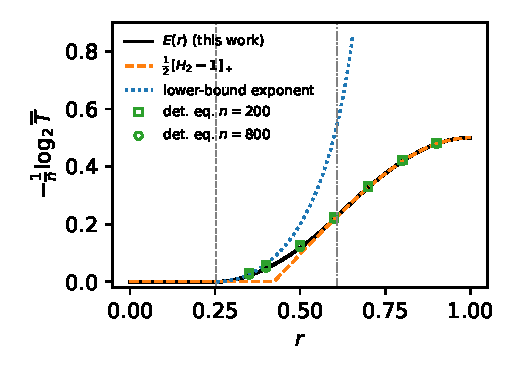
\includegraphics[width=0.9\columnwidth]{fig2.pdf}
\caption{Decay exponent for depolarizing noise. Solid: rigorous upper-bound exponent $E(r)$, Eq.~\eqref{eq:E}. Dashed: collision-entropy exponent $\tfrac12[H_2-1]_+$. Dotted: rigorous lower-bound exponent $E_{\rm lb}$. Symbols: $-\frac1n\log_2\Tb$ from the deterministic equivalent at $n=200,800$; finite-$n$ extrapolation agrees with $E(r)$ to $\lesssim2\times10^{-4}$. Vertical lines: hashing point $r_c$ and freezing point $r^\star$.}
\label{fig:2}
\end{figure}

\emph{Tightness: deterministic equivalent and exact numerics.}---For Haar states the vectors $\sqrt{p(P)}\,P|\psi_i\rangle$ have overlaps $O(d^{-1/2})$. This suggests replacing $\N(\psi_1)-\N(\psi_2)$ by $WDW^\dagger$, where $W$ is a $d\times 2\cdot4^n$ Gaussian matrix and $D=\mathrm{diag}(p,-p)$. The spectrum of this operator follows from the Silverstein--Bai equation~\cite{SilversteinBai}. Using $|x|=\frac2\pi\int_0^\infty\frac{x^2}{x^2+\tau^2}d\tau$ on the imaginary axis, we obtain
\begin{equation}
\Tb_{\rm DE}=\frac d\pi\int_0^{\mu_0}\!2\mu^2S(\mu)\Big|\frac{d\tau}{d\mu}\Big|d\mu,\quad
\tau=\frac1\mu-2\mu S(\mu),
\label{eq:DE}
\end{equation}
where $S(\mu)=d^{-1}\sum_Pp(P)^2/[1+p(P)^2\mu^2]$ and $\tau(\mu_0)=0$. For local noise, Eq.~\eqref{eq:DE} reduces to a sum over the $n+1$ Hamming weights and can be evaluated in log space for $n\sim10^3$. Exact simulations for $n\le10$ approach $\Tb_{\rm DE}$ with a relative deviation that shrinks roughly as $d^{-1/2}$; at $n=10$ it is at most $2\%$ for $r\le0.5$ [Fig.~\ref{fig:1}(a)]. In the frozen phase the deterministic equivalent reproduces the exponent but not the prefactor: at $n=10$, $r=0.9$ it even exceeds the rigorous bound by a factor of $1.7$, so we use it only for exponents there. In both phases, the large-$n$ exponents extracted from Eq.~\eqref{eq:DE} reproduce Eq.~\eqref{eq:E} to $\lesssim2\times10^{-4}$. Examples: $0.0216$ vs $0.0214$ at $r=0.35$, $0.1177$ vs $0.1176$ at $r=0.5$, and $0.3275$ vs $0.3276$ at $r=0.7$. In the frozen phase, exact data at $n=8,10$ and $r=0.7,0.9$ stay at a constant fraction, $0.78$--$0.81$, of the second-moment bound. This shows that the bound is tight up to an $O(1)$ prefactor. We therefore conjecture that $E(\bm p)$ in Eq.~\eqref{eq:E} is the exact decay exponent for all $\bm p$. This is proven at the transition and supported by both numerical methods elsewhere.

\emph{Discussion.}---We have shown that the distinguishability of scrambled states under Pauli noise is governed by the information spectrum of the noise. The result is a simple statement: two scrambled states survive the noise if and only if the error that occurred is among the $2^n$ most likely errors. This statement replaces entropic thresholds that hold only on average with a nonasymptotic identity, accurate up to $2^{-a/2}$ corrections. It fixes the transition at the hashing point and removes the intermediate phase. It also exposes a freezing transition in the decay rate that no single R\'enyi entropy captures.

Several implications follow. First, many proposals use random or pseudorandom states to encode information in noisy hardware~\cite{Bansal,Arute,Morvan}. For such proposals the relevant figure of merit is the coherent information, not the purity or the collision entropy. Below the hashing point no noise-robustness argument based on scrambling can apply. Second, because Theorem~1 needs no independence, it applies directly to correlated noise, for example noise produced by a noisy circuit after twirling. There the threshold becomes the point at which the surprisal spectrum crosses $n$. Third, the bound is an operator-level counterpart of decoupling theorems~\cite{Dupuis,HaydenPreskill}, now with matching constants on both sides. Extending the information-spectrum characterization to non-Pauli channels and to approximate designs generated by shallow circuits, where Ref.~\cite{Liu2026} reports polynomial floors, are natural next steps. Proving Eq.~\eqref{eq:E} tight in the large-deviation phase likely requires a measurement that is better than the subspace projector used here.

\emph{Code availability.}---Scripts that reproduce all figures and numbers are included with this manuscript.

\begin{thebibliography}{99}
\bibitem{HaydenPreskill} P. Hayden and J. Preskill, J. High Energy Phys. 09 (2007) 120.
\bibitem{Dalzell} A. M. Dalzell, N. Hunter-Jones, and F. G. S. L. Brand\~ao, Commun. Math. Phys. \textbf{405}, 78 (2024).
\bibitem{Bansal} N. Bansal, W.-K. Mok, K. Bharti, D. E. Koh, and T. Haug, PRX Quantum \textbf{6}, 020322 (2025).
\bibitem{Liu2026} G. Liu, C. Qin, Z. Xu, X. Ma, and Z.-W. Liu, arXiv:2606.02122 (2026).
\bibitem{Sommers} G. M. Sommers, J. A. Jacoby, Z. Weinstein, D. A. Huse, and S. Gopalakrishnan, PRX Quantum \textbf{7}, 020328 (2026).
\bibitem{VerduHan} S. Verd\'u and T. S. Han, IEEE Trans. Inf. Theory \textbf{40}, 1147 (1994).
\bibitem{HayashiNagaoka} M. Hayashi and H. Nagaoka, IEEE Trans. Inf. Theory \textbf{49}, 1753 (2003).
\bibitem{BDSW} C. H. Bennett, D. P. DiVincenzo, J. A. Smolin, and W. K. Wootters, Phys. Rev. A \textbf{54}, 3824 (1996).
\bibitem{Devetak} I. Devetak, IEEE Trans. Inf. Theory \textbf{51}, 44 (2005).
\bibitem{Webb} Z. Webb, Quantum Inf. Comput. \textbf{16}, 1379 (2016).
\bibitem{Zhu} H. Zhu, Phys. Rev. A \textbf{96}, 062336 (2017).
\bibitem{Derrida} B. Derrida, Phys. Rev. B \textbf{24}, 2613 (1981).
\bibitem{SilversteinBai} J. W. Silverstein and Z. D. Bai, J. Multivariate Anal. \textbf{54}, 175 (1995).
\bibitem{Arute} F. Arute \emph{et al.}, Nature \textbf{574}, 505 (2019).
\bibitem{Morvan} A. Morvan \emph{et al.}, Nature \textbf{634}, 328 (2024).
\bibitem{Dupuis} F. Dupuis, M. Berta, J. Wullschleger, and R. Renner, Commun. Math. Phys. \textbf{328}, 251 (2014).
\end{thebibliography}
\end{document}
